\clearpage
\section{Tiền xử lý dữ liệu}
\subsection{Làm sạch dữ liệu}
% Cách xử lý các giá trị bị thiếu (Missing values) và loại bỏ nhiễu/ngoại lệ (Outliers - ví dụ: dùng phương pháp IQR).
Sử dụng lệnh \texttt{df.columns[df.isnull().any()]} ta thấy được các cột có giá trị khuyết.
\begin{figure}[H]
    \centering
    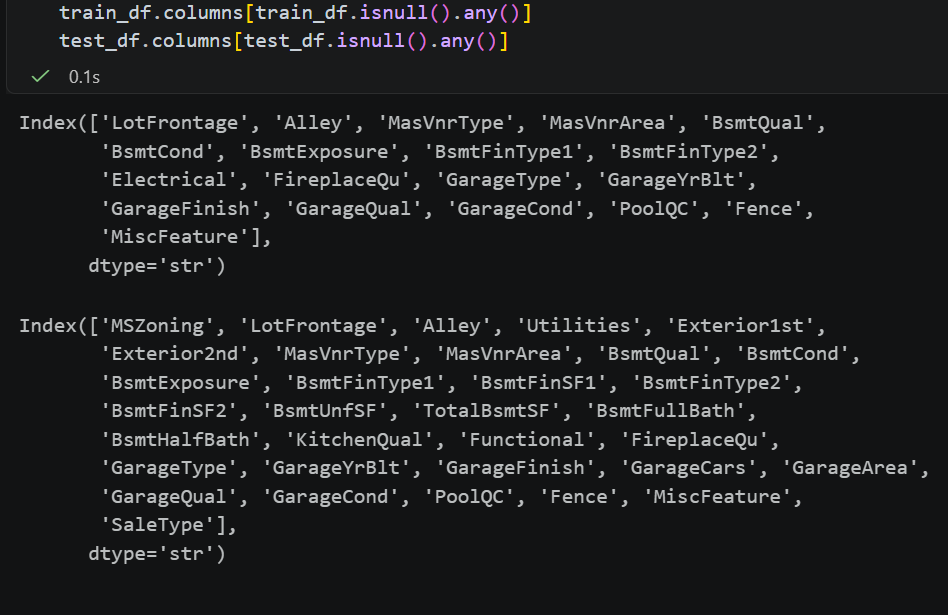
\includegraphics[width=1\linewidth]{images/preprocess/image.png}
    \caption{Danh sách cột bị thiếu}
\end{figure}
Dễ thấy tập dữ liệu đang có rất nhiều thuộc tính đang có dữ liệu bị thiếu. Đặc biệt khi dùng \texttt{df.info()} ta thấy PoolQC chỉ có 3 giá trị. Để đảm bảo tính toàn vẹn của dữ liệu trước khi đưa vào mô hình huấn luyện, nhóm đã thực hiện quy trình xử lý giá trị thiếu  dựa trên đặc thù ý nghĩa của từng nhóm thuộc tính. Quy trình cụ thể như sau:

\subsubsection{Xử lý theo nhóm đặc tính}
\begin{itemize}[label=\textendash, leftmargin=3em]
    \item[-] \textbf{Nhóm thuộc tính tiện ích:} Đối với các biến như PoolQC, MiscFeature, Alley, Fence, FireplaceQu và các biến liên quan đến Garage, Basement, giá trị thiếu được điền là "None". Phản ánh thực tế rằng căn nhà đó không có các tiện ích tương ứng 
    \item[-] \textbf{Nhóm thuộc tính số học:} Các biến như GarageCars, GarageArea, BsmtFinSF1, BsmtFinSF2, TotalBsmtSF, BsmtFullBath... được điền bằng giá trị 0 nếu dữ liệu bị khuyết.
    \item[-] \textbf{Điền theo giá trị phổ biến:} Với các biến có mang tính chất phân loại khu vực như MSZoning, Electrical, Exterior1st, KitchenQual, SaleType, giá trị xuất hiện thường xuyên nhất của cột đó được sử dụng để lấp đầy khoảng trống.
\end{itemize}

\subsubsection{Xử lý theo logic phụ thuộc và thống kê khu vực}
\indent Một số thuộc tính đòi hỏi phương pháp xử lý phức tạp hơn để giữ được tính phân hóa của dữ liệu:
\begin{itemize}[label=\textendash, leftmargin=3em]
    \item[-] \textbf{LotFrontage (Chiều dài mặt tiền):} Do kích thước mặt tiền thường tương đồng trong cùng một khu vực, nhóm sử dụng giá trị trung vị của các căn nhà trong cùng Neighborhood để điền vào các vị trí thiếu.
    \item[-] \textbf{GarageYrBlt (Năm xây gara):} Trong trường hợp giá trị này bị thiếu, nhóm giả định gara được xây cùng lúc với căn nhà và sử dụng giá trị của cột \textit{YearBuilt} để thay thế.
    \item[-] \textbf{MasVnr (Lớp vỏ trang trí):} Nhóm áp dụng xử lý có điều kiện:
    \begin{itemize}
        \item[+] Nếu MasVnrArea $> 0$ nhưng loại vỏ Type bị thiếu, điền loại vỏ phổ biến nhất khác "None".
        \item[+] Nếu diện tích Area bị thiếu nhưng đã có loại vỏ, sử dụng diện tích trung bình của loại vỏ đó để điền vào.
        \item[+] Các trường hợp còn lại mặc định về "None" và 0.
    \end{itemize}
\end{itemize}

\subsubsection{Xử lý theo nhóm đặc tính}
\begin{itemize}[label=\textendash, leftmargin=3em]
    \item[-] \textbf{Nhóm thuộc tính tiện ích:} Đối với các biến như PoolQC, MiscFeature, Alley, Fence, FireplaceQu và các biến liên quan đến Garage, Basement, giá trị thiếu được điền là "None". Phản ánh thực tế rằng căn nhà đó không có các tiện ích tương ứng 
    \item[-] \textbf{Nhóm thuộc tính số học:} Các biến như GarageCars, GarageArea, BsmtFinSF1, BsmtFinSF2, TotalBsmtSF, BsmtFullBath... được điền bằng giá trị 0 nếu dữ liệu bị khuyết.
    \item[-] \textbf{Điền theo giá trị phổ biến:} Với các biến có mang tính chất phân loại khu vực như MSZoning, Electrical, Exterior1st, KitchenQual, SaleType, giá trị xuất hiện thường xuyên nhất của cột đó được sử dụng để lấp đầy khoảng trống.
\end{itemize}
\subsection{Chuyển đổi dữ liệu}

\indent Sau khi xử lý các giá trị thiếu, các thuộc tính phân loại cần được chuyển đổi sang dạng số để các thuật toán máy học có thể tính toán. Trong bài toán này, nhóm đã áp dụng hai chiến lược mã hóa khác nhau tùy thuộc vào bản chất của dữ liệu:

\subsubsection{Mã hóa thứ tự (Ordinal Encoding)}
\indent Một đặc điểm quan trọng của tập dữ liệu giá nhà Ames là có rất nhiều thuộc tính thể hiện mức độ đánh giá (ví dụ: Chất lượng từ "Tồi" đến "Xuất sắc"). Để giữ được mối quan hệ thứ bậc này, nhóm đã thực hiện ánh xạ thủ công các giá trị chữ thành các con số tương ứng.

\begin{itemize}
    \item[-] \textbf{Nhóm đánh giá chất lượng:} Các biến như ExterQual, HeatingQC, KitchenQual... được ánh xạ từ 0 đến 5 tương ứng với các mức độ: \textit{None} (0), \textit{Po} (1), \textit{Fa} (2), \textit{TA} (3), \textit{Gd} (4), \textit{Ex} (5).
    \item[-] \textbf{Nhóm đặc tính kỹ thuật:}
    \begin{itemize}
        \item[+] \textit{BsmtFinType}: Được mã hóa từ 0 (None) đến 6 (GLQ).
        \item[+] \textit{Functional}: Mã hóa mức độ hoạt động của căn nhà từ 0 (Sal - hư hỏng nặng) đến 7 (Typ - bình thường).
        \item[+] \textit{CentralAir, PavedDrive, Fence}: Chuyển đổi sang dạng số dựa trên sự tồn tại hoặc mức độ kiên cố của tiện ích.
    \end{itemize}
\end{itemize}

\subsubsection{Mã hóa biến giả (One-Hot Encoding)}
\indent Đối với các biến phân loại còn lại không có tính chất thứ bậc rõ rệt (ví dụ: Neighborhood, MSZoning, Foundation), nhóm sử dụng phương pháp One-Hot Encoding chuyển giá trị phân loại thành một cột riêng biệt với giá trị nhị phân (0 hoặc 1). Nhóm đã sử dụng tham số \texttt{drop\_first=True} để loại bỏ cột đầu tiên trong mỗi nhóm biến mới, nhằm tránh hiện tượng đa cộng tuyến (Multicollinearity).
\subsection{Chuẩn hóa dữ liệu}
%Sử dụng StandardScaler để đưa các đặc trưng số học về cùng thang đo.
\indent Nhóm sử dụng kỹ thuật \texttt{StandardScaler} để đưa các thuộc tính số học về cùng một thang đo với trung bình bằng 0 và độ lệch chuẩn bằng 1. Công thức chuẩn hóa:
\begin{equation}
z = \frac{x - \mu}{\sigma}
\end{equation}
Để tránh rò rỉ thông tin (Data Leakage), chúng ta sử dụng \texttt{fit()} trên tập huấn luyện rồi transform trên cả hai tập dữ liệu thay vì gộp hai tập dữ liệu rồi chuẩn hóa.
\subsection{Trích xuất đặc trưng}
Nhằm giúp các mô hình dự đoán học tốt và cho kết quả tốt hơn. Nhóm tiến hành trích xuất và lựa chọn đặc trưng:

\subsubsection{Loại bỏ các thuộc tính ít giá trị}
\indent Nhóm thực hiện loại bỏ các cột dữ liệu có tỉ lệ khuyết thiếu quá cao hoặc độ lệch dữ liệu (\textit{data imbalance}) quá lớn như: \textit{Utilities, Street, PoolQC, LowQualFinSF}. Việc loại bỏ các biến "nhiễu" này giúp mô hình tập trung vào các thuộc tính thực sự có khả năng giải thích sự biến động của giá nhà.
\begin{figure}[htbp]
    \centering
    \begin{minipage}{0.32\textwidth}
        \centering
        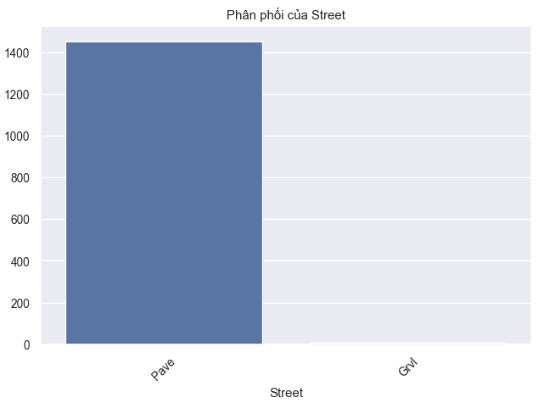
\includegraphics[width=\linewidth]{images/preprocess/street.png}
    \end{minipage}
    \hfill 
    \begin{minipage}{0.32\textwidth}
        \centering
        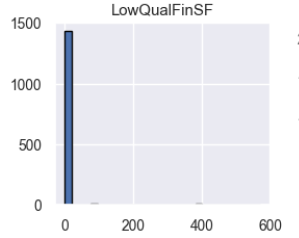
\includegraphics[width=\linewidth]{images/preprocess/lowQualFsh.png}
    \end{minipage}
    \hfill
    \begin{minipage}{0.32\textwidth}
        \centering
        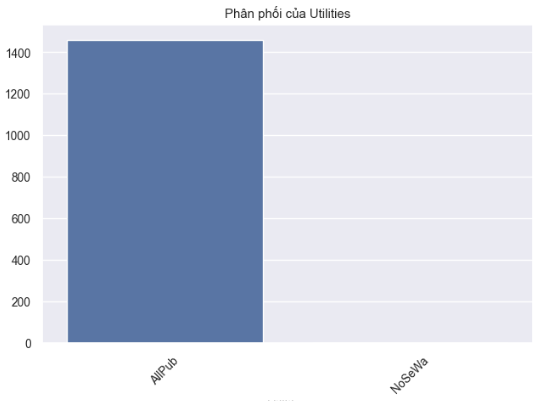
\includegraphics[width=\linewidth]{images/preprocess/utility.png}
    \end{minipage}
    \vspace{0.2cm}
    \caption{Thống kê của các thuộc tính bị loại.}
\end{figure}
\subsubsection{Tạo lập các biến tổng hợp}
\indent Thay vì để các thông số rời rạc, nhóm xây dựng các biến tổng hợp nhằm phản ánh quy mô toàn diện của căn nhà:
\begin{itemize}[label=\textendash, leftmargin=3em]
    \item[-] \textbf{TotalSF (Tổng diện tích):} Được tính bằng tổng diện tích tầng hầm TotalBsmtSF, tầng một 1stFlrSF và tầng hai 2ndFlrSF.
    \item[-] \textbf{Total\_Bathrooms (Tổng số phòng tắm):} Nhóm thực hiện quy đổi các phòng tắm phụ HalfBath thành 0.5 đơn vị để tạo ra một biến số thực thể hiện chính xác tiện nghi của căn nhà.
\end{itemize}

\subsubsection{Đặc trưng về thời gian và trạng thái}
\begin{itemize}[label=\textendash, leftmargin=3em]
    \item[-] \textbf{HouseAge và RemodAge:} Thay vì sử dụng năm xây dựng gốc, nhóm tính toán "Tuổi thọ" của căn nhà và khoảng thời gian từ lần sửa chữa cuối cùng đến khi bán. Nhà càng mới hoặc vừa mới sửa chữa thường có giá trị cao hơn.
    \item[-] \textbf{Biến trạng thái (Boolean):} Chuyển đổi các cột số lượng thành các biến đánh dấu \texttt{0} hoặc \texttt{1} (Ví dụ: \textit{HasFireplace}) để mô hình dễ dàng nhận diện sự hiện diện của các tiện ích cao cấp.
\end{itemize}
\subsubsection{Biến tương tác}
\indent Để nắm bắt các mối quan hệ phi tuyến tính, nhóm tạo ra các biến như \texttt{Qual\_x\_TotalSF}. Điều này dựa trên thực tế rằng diện tích lớn chỉ thực sự có giá trị cao khi đi kèm với chất lượng xây dựng tốt. 
\subsubsection{Giảm lệch}
Cuối cùng, nhóm áp dụng Log Transformation cho các biến diện tích (\textit{TotalSF, GrLivArea, LotArea}) để giảm độ lệch, 